% Shared standalone design for the editable figure reconstructions.
\documentclass[tikz,border=5pt,10pt]{standalone}
\usepackage[T1]{fontenc}
\usepackage[utf8]{inputenc}
\usepackage{newpxtext,newpxmath}
\usepackage[scaled=.94]{sourcesanspro}
\usepackage{pgfplots}
\pgfplotsset{compat=1.18}
\usetikzlibrary{arrows.meta,calc,positioning,decorations.pathreplacing,
  decorations.markings,patterns,matrix,shapes.geometric,fit,backgrounds,
  intersections,angles,quotes}
\definecolor{ink}{HTML}{203746}
\definecolor{accent}{HTML}{146C78}
\definecolor{muted}{HTML}{667780}
\definecolor{signalred}{HTML}{B94B44}
\color{ink}
\tikzset{>=Latex,line width=.8pt,
  every node/.style={font=\small},
  axis/.style={->,draw=muted,line width=.5pt},
  guide/.style={draw=muted,dashed,line width=.45pt},
  curve/.style={draw=accent,line width=1pt},
  marker/.style={circle,fill=accent,inner sep=1.5pt},
  labelbox/.style={fill=white,inner sep=2pt}}

\begin{document}
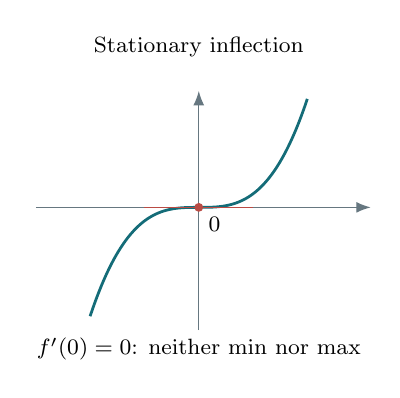
\begin{tikzpicture}[x=1.15cm,y=.8cm,every node/.style={font=\footnotesize}]
\draw[axis] (-1.8,1.3)--(1.9,1.3);\draw[axis] (0,-.65)--(0,3.15);
\draw[curve,domain=-1.2:1.2,samples=150] plot (\x,{\x^3+1.3});
\draw[signalred] (-.6,1.3)--(.6,1.3);\fill[signalred] (0,1.3) circle(1.6pt);
\node[below right] at (0,1.3) {$0$};
\node at (0,3.85) {Stationary inflection};\node at (0,-.95) {$f'(0)=0$: neither min nor max};
\end{tikzpicture}
\end{document}
